\documentclass{article}
\usepackage[utf8]{inputenc}
\usepackage[osf,sc]{mathpazo}
\usepackage[scaled=0.90]{helvet}
\usepackage[table,dvipsnames]{xcolor}
\usepackage[breaklinks]{hyperref}

\usepackage{enumitem,mathtools}
% \usepackage[ruled,vlined]{algorithm2e}
\usepackage[ruled,vlined,resetcount]{algorithm2e}

% \SetAlFnt{\small}
\usepackage{algorithmic}

\usepackage{float}
\usepackage{soul}
\usepackage{subcaption}
\usepackage[capitalise]{cleveref}
\usepackage{graphicx}
\usepackage{lineno}
\usepackage{url}
% \def\UrlBreaks{\do\/\do-}

% \usepackage{breakurl}
\usepackage[breaklinks]{hyperref}

\usepackage{tcolorbox}
\usepackage{array}
\usepackage{tabularx}

\hypersetup{
    colorlinks=true,
    linkcolor=cyan, % color1 : will be black
    filecolor=red,
    urlcolor=ForestGreen,
    citecolor=red,
    bookmarksopen=false,
    pdftitle={Title},
    pdfauthor={Author},
}

\definecolor{darkpastelpurple}{rgb}{0.59, 0.44, 0.84}
\def\code#1{\textbf{\texttt{#1}}}
\def\codeRed#1{{\color{Maroon}{\textbf{\texttt{#1}}}}}
\def\codeCyan#1{{\color{cyan}{\textbf{\texttt{#1}}}}}
\def\vari#1{{\color{Cerulean}{\textbf{\texttt{#1}}}}}
\def\func#1{{\color{Purple}{\textbf{\texttt{#1}}}}}
\newenvironment{coded}{\color{blue}\code}

\definecolor{Gray}{gray}{0.95}
\colorlet{shadecolor}{gray!40}
\definecolor{LightCyan}{rgb}{0.88, 1, 1}
%\definecolor{LightCyan}{rgb}{0.92, 0.98, 0.98}
\definecolor{brickred}{rgb}{0.8, 0.25, 0.33}
\definecolor{mgreen}{rgb}{0.2, 0.8, 1}
\definecolor{bleudefrance}{rgb}{0.19, 0.55, 0.91}
\definecolor{aliceblue}{rgb}{0.94, 0.97, 1.0}
\definecolor{azureWeb}{rgb}{0.94, 1.0, 1.0}
\definecolor{beaublue}{rgb}{0.74, 0.83, 0.9}
\definecolor{gainsboro}{rgb}{0.86, 0.86, 0.86}
\definecolor{linen}{rgb}{0.98, 0.94, 0.9}
\definecolor{oldlace}{rgb}{0.99, 0.96, 0.9}
\definecolor{magnolia}{rgb}{0.97, 0.96, 1.0}
\definecolor{moccasin}{rgb}{0.98, 0.92, 0.84}
\definecolor{navajowhite}{rgb}{1.0, 0.87, 0.68}
\definecolor{palecornflowerblue}{rgb}{0.67, 0.8, 0.94}


\usepackage{enumitem}
\setlist[description]{%
  topsep=10pt,   % space before start / after end of list
% itemsep=5pt,   % space between items
%   font={\bfseries\sffamily}, % set the label font
%  font={\bfseries\sffamily\color{red}}, % if colour is needed
font={\color{red}},
}

\newcommand{\EVI}{E\!V\!I}
\newcommand{\NDVI}{N\!D\!V\!I}
\newcommand{\NIR}{N\!I\!R}

\title{Google Earth Engine}
\author{Hossein Noorazar}
\date{\today}

\begin{document}
\maketitle
\tableofcontents

\clearpage

\section{Preface}
Google Earth Engine sucks! 
Below (Fig.~\ref{fig:GEESucks}) 
we have a simple example to show GEE is very specific.
Accessing to elements/entries of its object is not
intuitive. Figuring out every single step is a 
challenge.
\begin{figure}[H]
  \centering
  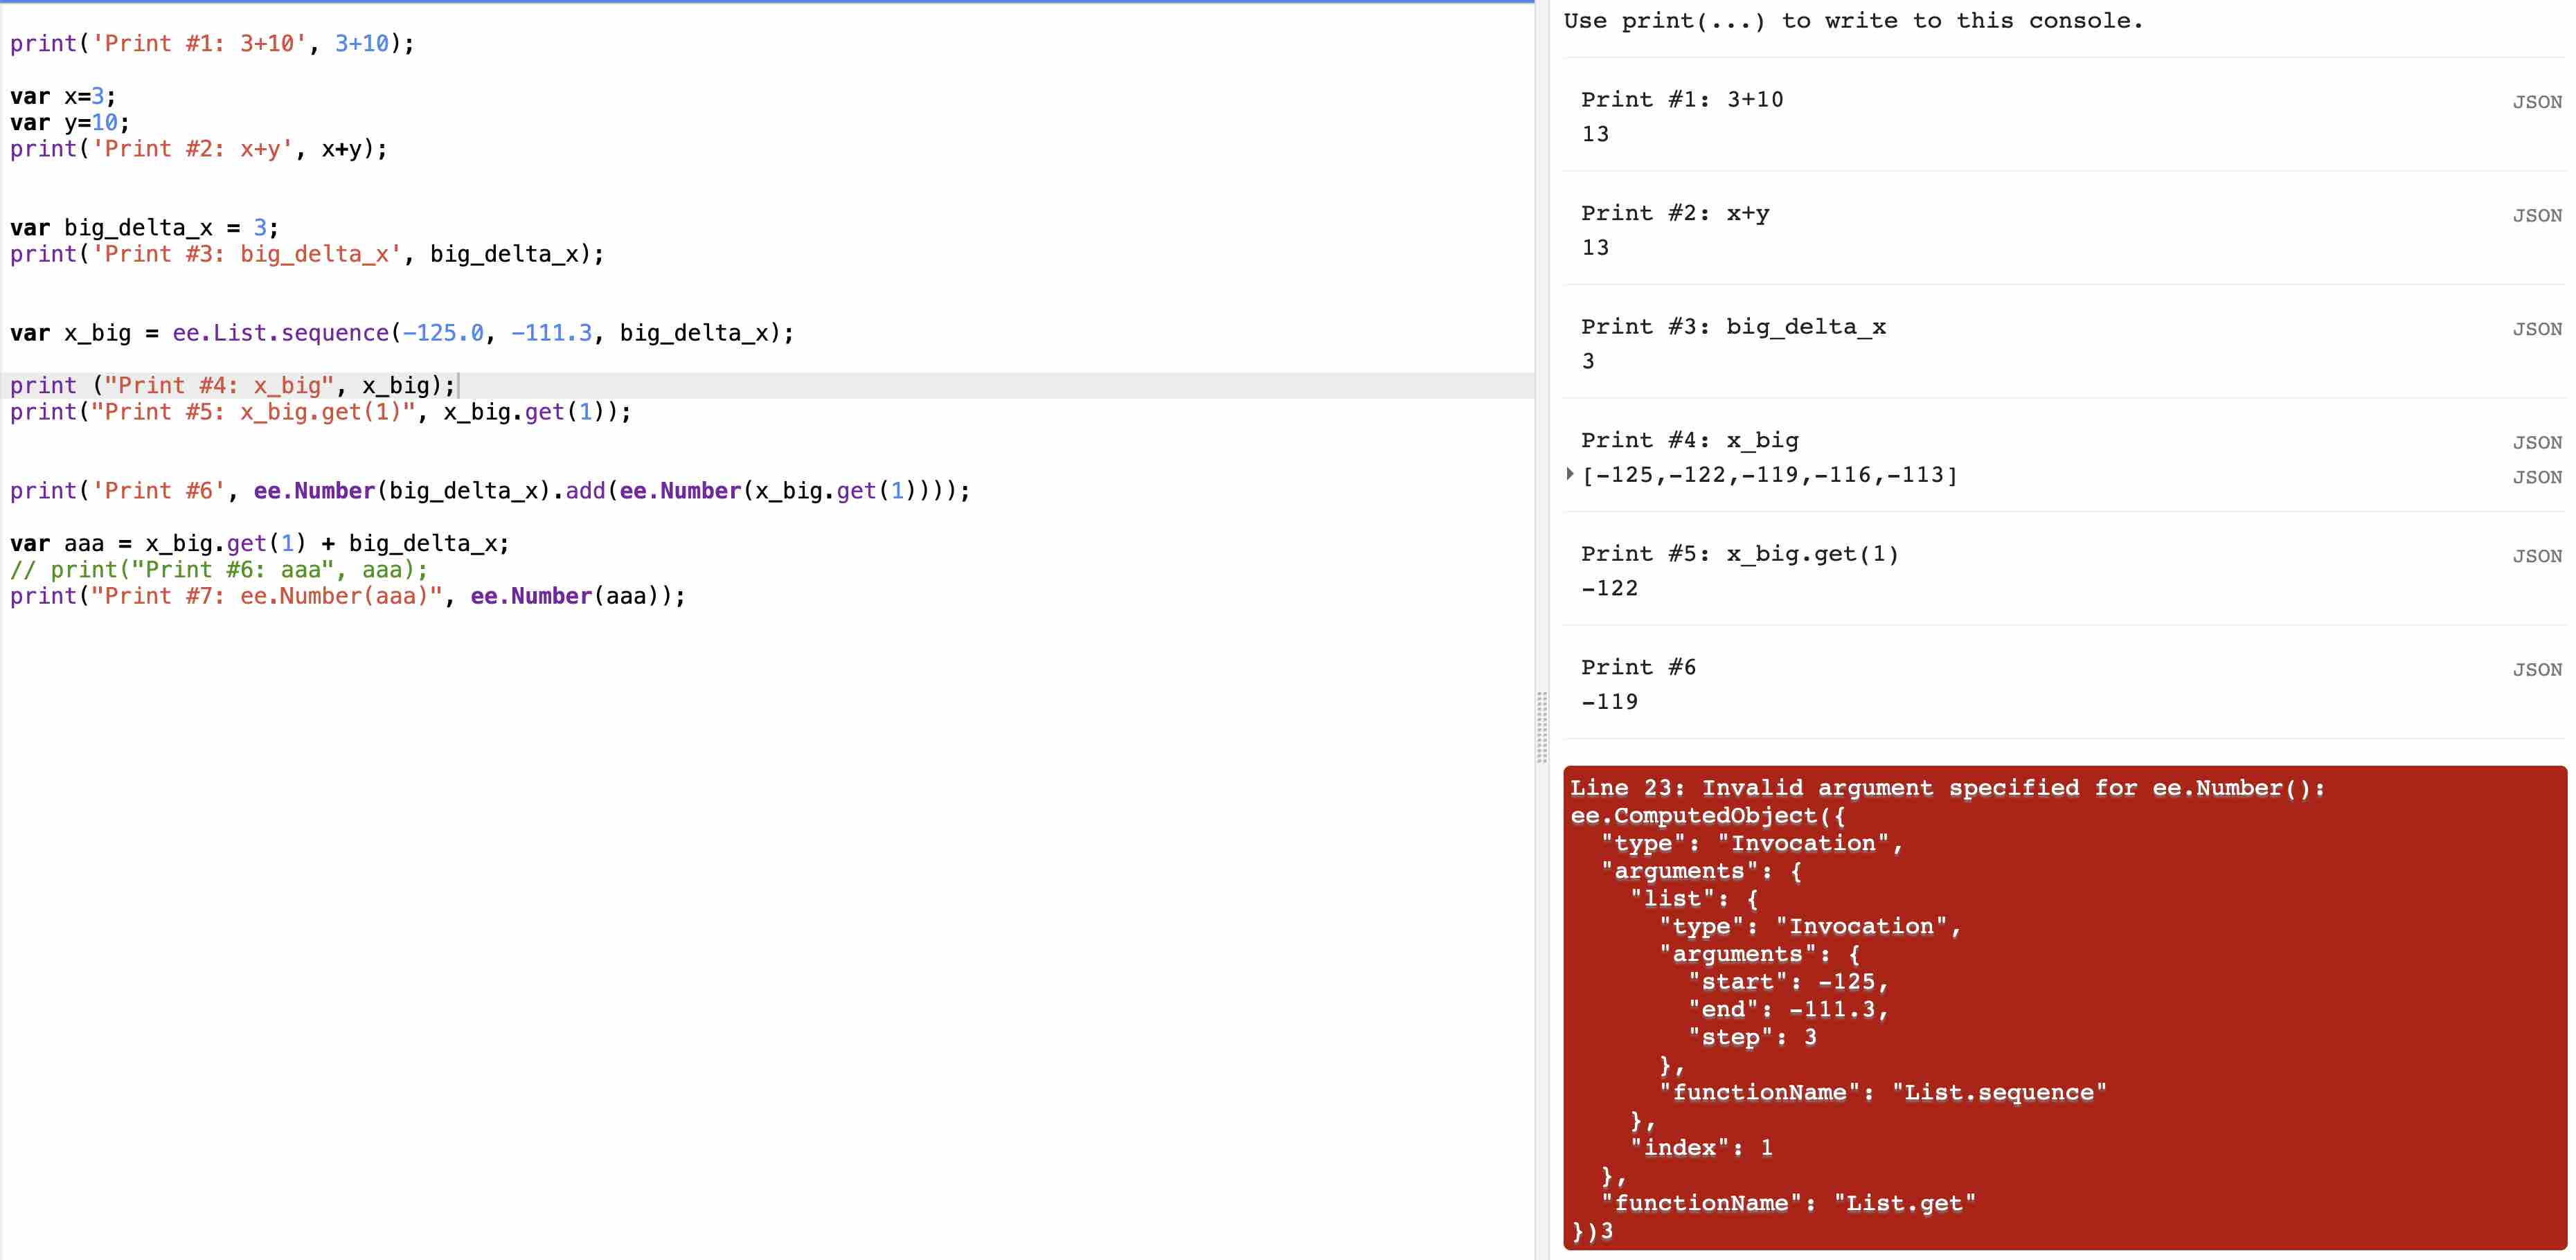
\includegraphics[width=1\textwidth]{figures/GEE_Sucks}
  \caption{GEE sucks.}
  \label{fig:GEESucks}
\end{figure}

\noindent Here is the code used for generation of Fig.~\ref{fig:GEESucks}.
\begin{tcolorbox}
%  \textbf{Algorithm for gradient descent with momentum is given below}
  \begin{algorithm}[H]
  \label{alg:GEE_Sucks}
   \caption{GEE Sucks.}
\SetAlgoLined
% \KwResult{Faster convergence}
1. \func{print}(\codeRed{``Print \#1: 3+10''},~\vari{3+10}) \;
2. \textbf{var} \code{x=}\vari{3}  \;
3. \textbf{var} \code{y=}\vari{10} \;
4. \func{print}(\codeRed{``Print \#2: x+y''}, 
\code{x+y}) \;
\vspace{.1in}
5. \textbf{var} \code{big\_delta\_x} = \vari{3} \;
6. \func{print}(\codeRed{``Print \#3: big\_delta\_x''}, \code{big\_delta\_x}) \;
\vspace{.1in}
7. \textbf{var} \code{x\_big} = \func{ee.List.sequence}(\vari{-125.0},~\vari{-111.3}, \code{big\_delta\_x}) \;
\vspace{.1in}
8. \func{print} (\codeRed{``Print \#4: x\_big''}, \code{x\_big}) \;
9. \func{print}(\codeRed{``Print \#5: x\_big.get(1)''}, \code{x\_big}.\func{get}(\vari{1})) \;
10. \func{print}(\codeRed{``Print \#6''},

\func{\textbf{ee.Number}}(\code{big\_delta\_x}).\func{add}
(\func{\textbf{ee.Number}}(\code{x\_big}.\func{get}(\vari{1})))) \;
\vspace{.1in}
11. \textbf{var} \code{aaa} 
     = \code{x\_big}.\func{get}(\vari{1}) +
     \code{big\_delta\_x} \;
12. // \func{print}(\codeRed{``Print \#7: aaa''}, \code{aaa}) \; 
13. \func{print}(\codeRed{``Print \#8: ee.Number(aaa)''}, \func{\textbf{ee.Number}}(\code{aaa})) \;
\end{algorithm}
\end{tcolorbox}

%%%%%%%----------------------------------------
%%%%%%%
%%%%%%%  JS or Python Interface
%%%%%%%
\section{JavaScript or Python Interface}
I think Python should be avoided in
this particular case for the following reasons:
\begin{enumerate}
    \item The interface is too slow,
    \item The interface needs authentication every 
          single time,
    \item Google does not maintain the Python. Therefore,
          the functions are first written/updated for
          the JavaScript (JS) by Google,
          and the Python
          equivalents/updates will not be provided 
          in a timely manner (who knows when?).
    \item The tutorials for JS is already 
          hard to find, it is much worse for Python. 
          Again, since Google is responsible for
          JavaScript, it releases the
          tutorials for it, but not Python.
          
          P.S. tutorials for JS might be abundant,
          but finding your exact needs might be hard.
          Even when you find something you may not
          be sure if that is the best possible
          solution.
\end{enumerate}

%%%%%%%--------------------------------------------------------------------------
%%%%%%%
%%%%%%%  Landsat Products and Differences
%%%%%%%
\section{Landsat Products and Differences}

There are different products\footnote{start here to collect some information. some of the products are deprecated and superseded and Google does not show them easily: \href{https://developers.google.com/earth-engine/datasets/catalog/landsat}{here}} that fall under 
different labels; tier 1 vs tier 2, collection 1 vs collection 2, level 1 and level 2.
Some of these have the same description on 
Google developer pages. For example, 
\href{https://developers.google.com/earth-engine/datasets/catalog/LANDSAT_LC08_C01_T1_SR#description}{USGS Landsat 8 Surface Reflectance Tier 1}
and \href{https://developers.google.com/earth-engine/datasets/catalog/LANDSAT_LC08_C01_T2_SR#description}{USGS Landsat 8 Surface Reflectance Tier 2}
have the same description and identical bands. In this particular example
we want to use Tier 1. But we need a deeper understanding of differences(?)

Based on the information below and references therein, Collection 2 is an improvement
over Collection 1\footnote{Is there any time period for which Collection 2 
does not exist but 1 does?}.
It seems Collection-2 Level-2 Tier-1 should be the best, but
in our plots it was not different from T1\_SR (\cref{fig:C2L2Performance}). 
Also keep in mind \hl{Collection-2 Level-2 bands must be scaled.}

\begin{figure}[H]
  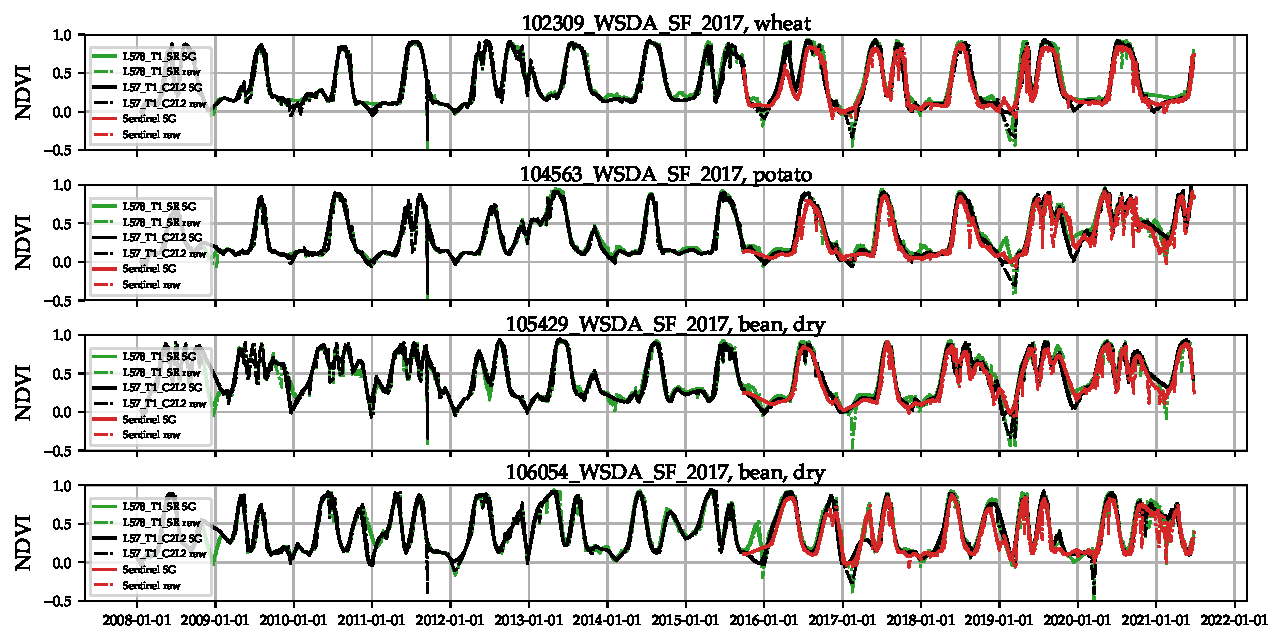
\includegraphics[width=1\textwidth]{figures/00_merged_Landsats_Smoothed_and_raw}
\caption{In this plot the data points from Landsat-5, -7, and -8 (Tier 1, Surface Reflectance, from GEE collection LANDSAT/LE07/C01/T1\_SR) are
merged together to form one vector. The same is done to Landsat-5 and -7 Collection-2 Level-2 (from GEE collection LANDSAT/LE07/C02/T1\_L2).}
We can see they all are performing well.
\label{fig:C2L2Performance}
\end{figure}


Moreover, GEE~\cite{Landsat7T1SRBandWidths}
says ``This dataset is the atmospherically corrected surface
reflectance from the Landsat 7 ETM+ sensor.'' about ``USGS Landsat 7 
Surface Reflectance Tier 1''  (LANDSAT/LE07/C01/T1\_SR). 
On the other hand, it also says ``Caution: 
This dataset has been superseded by LANDSAT/LC08/C02/T1\_L2.'' 

Collection-1 has only Level-1 data, however, Collection-2 has 
level-1 as well as Level-2.


\begin{description}
\item [Collection 1] Landsat Collection 1 was established in 2016 to improve archive management.
\href{https://www.usgs.gov/core-science-systems/nli/landsat/landsat-collection-1?qt-science_support_page_related_con=1#qt-science_support_page_related_con}{Learn more about Collection 1 from the USGS.}

Landsat Collection 1 consists of Level-1 data products 
generated from Landsat 8 Operational Land Imager (OLI)/Thermal 
Infrared Sensor (TIRS), Landsat 7 Enhanced Thematic Mapper 
Plus (ETM+), Landsat 4-5 Thematic Mapper (TM)*, and Landsat 1-5 
Multispectral Scanner (MSS) instruments.
\textbf{Collection 1 Tiers:}
\begin{description}
\item [Tier 1]
``Landsat scenes with the highest available data quality are placed into 
Tier 1 and are considered suitable for time-series analysis.''~\cite{C1Describe}

\item [Tier 2] ``Landsat scenes not meeting Tier 1 criteria during processing
 are assigned to Tier 2. Tier 2 scenes adhere to the same radiometric 
 standard as Tier 1 scenes, but do not meet the Tier 1 geometry 
 specification due to less accurate orbital information 
 (specific to older Landsat sensors), significant cloud cover, 
 insufficient ground control, or other factors.''~\cite{C1Describe}
\end{description}



\item [Collection 2] 
Landsat Collection 2 marks the second major reprocessing effort on 
the Landsat archive by the USGS that results in several data product 
improvements that harness recent advancements in data processing, 
algorithm development, and data access and distribution capabilities. 
\href{https://www.usgs.gov/core-science-systems/nli/landsat/landsat-collection-2?qt-science_support_page_related_con=1#}{Learn more about Collection 2 from the USGS.}

Collection-2 Level-1 has different processings for different satellites~\cite{C2L1Describe}.
It seems Collection-2 level-1 is TOA and Collection-2 level-2 is Surface Reflectance. 
``Collection-2 Level-2 science products are generated from Collection 2 Level-1 
inputs that meet the <76 degrees Solar Zenith Angle constraint and include the 
required auxiliary data inputs to generate a scientifically viable product.''~\cite{C2L2Describe}.
``\textbf{Surface reflectance} (unitless) 
measures the fraction of incoming solar radiation that is 
reflected from the Earth's surface to the Landsat sensor. 
The LEDAPS and LaSRC surface reflectance algorithms 
correct for the temporally, spatially and spectrally varying scattering 
and absorbing effects of atmospheric gases, aerosols, and water vapor, 
which is necessary to reliably characterize the Earth’s land surface.''~\cite{C2L2Describe}.
For the enhancement details please see~\cite{C2L2Describe}.
\end{description}






%%%%%%%--------------------------------------------------------------------------
%%%%%%%
%%%%%%%  Access a Feature/Entry of a FeatureCollection
%%%%%%%
\section{Access a Feature/Entry of a FeatureCollection}

Suppose your \code{featurecollection} 
is called \code{SF}.
In order to access its entries you have to
convert it to a \vari{list} and then use \func{get(.)}:\\

\func{print} (\codeRed{``SF.get(0)''},
\code{SF}.\func{toList}(\vari{4}).\func{get}(\vari{0}));\\

\noindent where \vari{4} is the size 
of \code{SF} known in advance, and
\vari{0} is index of first entry of \code{SF}. 
In general you can use:\\

\func{print} (\codeRed{``SF.get(0)''},
\code{SF}.\func{toList}(\vari{\code{SF}.\func{size}\code{()}}).\func{get}(\vari{index}));\\

\noindent Please note if you use 
\code{SF}.\func{get}(\codeCyan{0}) 
you will get an error.

%%%%%%%----------------------------------------
%%%%%%%
%%%%%%% 
%%%%%%%
\section{Add a Property to a Feature}

Suppose you have uploaded a shapefile \vari{SF}
into your assets. The shapefiles usually have a 
component/slice called \vari{data} (which is of type datatable) 
that can be
accessed via \vari{SF@data} in R. This component stores
metadata corresponding to each polygon.

Say each polygon is an agricultural field
that has some attributes associated with it such as irrigation type,
area of the field, etc. After some computations
on GEE you may want to attach these metadata to
the output to use later. These metadata is referred to
by \vari{properties} on GEE. If you want to manually add a
property to a feature you should use:\\

\code{a\_feature = a\_feature}.\func{set}(\codeRed{`my\_property'}, \codeRed{1});\\

If you want to copy \vari{properties} (metadata)
of \vari{feature\_b} into \vari{feature\_a} you can do:\\

\code{feature\_a} = \code{feature\_a}.\func{copyProperties}(\code{feature\_b}, [\codeRed{`ID`}, \codeRed{`Irrigation\_type'}]);\\

\noindent where [\codeRed{`ID`}, \codeRed{`Irrigation\_type'}] 
is a subset of \vari{properties} of \vari{feature\_b} 
to be copied into \vari{feature\_a}.
I guess if that argument is dropped, then
all \vari{properties} will be copied.


%%%%%%%----------------------------------------
%%%%%%%
%%%%%%% Find Centroid of Polygons
%%%%%%%
\section{Find Centroid of Polygons}
Suppose you have a shapefile that you have
uploaded to GEE as an \emph{asset}. Here
we will see how to find the centroids of
the polygons in the shapefile.
Let the name of shapefile be \vari{Our\_ShapeFile}.
The function to compute centroids of the
polygons in \vari{Our\_ShapeFile} is
given by Alg.~\ref{alg:FindCentroidsAPoly}\footnote{This algorithm is 
accessible on GEE \href{https://code.earthengine.google.com/df1685205d4fbfd8def0efb12a75f8e4}{here}.}.
Line 4 of the Alg.~\ref{alg:FindCentroidsAPoly}
is keeping the columns of data slice in \vari{Our\_ShapeFile}; 
\vari{Our\_ShapeFile}@data.
\begin{tcolorbox}
  \begin{algorithm}[H]
  \label{alg:FindCentroidsAPoly}
   \caption{Find Centroids of Polygons in a Shapefile.}
\SetAlgoLined
% \KwResult{Faster convergence}
1. \textbf{function} \code{getCentroid(feature)} \{ \\
  \vspace{.1in}
\hspace{.2in} 2. {\color{ForestGreen}{// Keep this list of properties.}}\;
\hspace{.2in} 3. \textbf{var} \code{keepProperties =} [\codeRed{`ID'}, \codeRed{`county'}] \;
  \vspace{.2in}
\hspace{.2in} 4. {\color{ForestGreen}{// Get the centroid of the feature's geometry.}}\;
\hspace{.2in} 5. \textbf{var} \code{centroid =} 
\code{feature}.\func{geometry}().\func{centroid}(); \;
  \vspace{.2in}
\hspace{.2in} 6. 
{\color{ForestGreen}{// Return a new Feature, 
copying properties from the
  
\hspace{0.5in} old Feature.}}\;
\hspace{.2in} 7. \textbf{return}
\func{ee.Feature}(\code{centroid}).\func{copyProperties}
     (\code{feature},
 
  \hspace{2.8in}\code{keepProperties})\;
8. \}
  
  \vspace{.1in}
9. \textbf{var} \code{SF =} \func{ee.FeatureCollection}(\code{Our\_ShapeFile})\;
10. \textbf{var} \code{centroids\_from\_GEE} = \code{SF}.\func{map}(\code{getCentroid});
\end{algorithm}
\end{tcolorbox}

{\color{red}{Warning:}} 
Imagine your polygon looks like a doughnut (non-convex shape).
Then the centroid would be in the center 
of the disk in the center
of the doughnut which is not part of the doughnut/polygon/region of interest.
So, if you want to look at an area around 
the centroid, then
that area (or parts of it, depending on how large the area is) 
would not belong to the polygon 
(See Fig.~\ref{fig:badBuffer}; it is not a doughnut, 
but it delivers the message!)
\begin{figure}[!h]
  \centering
  \begin{subfigure}[b]{0.4\textwidth}
    % \centering
    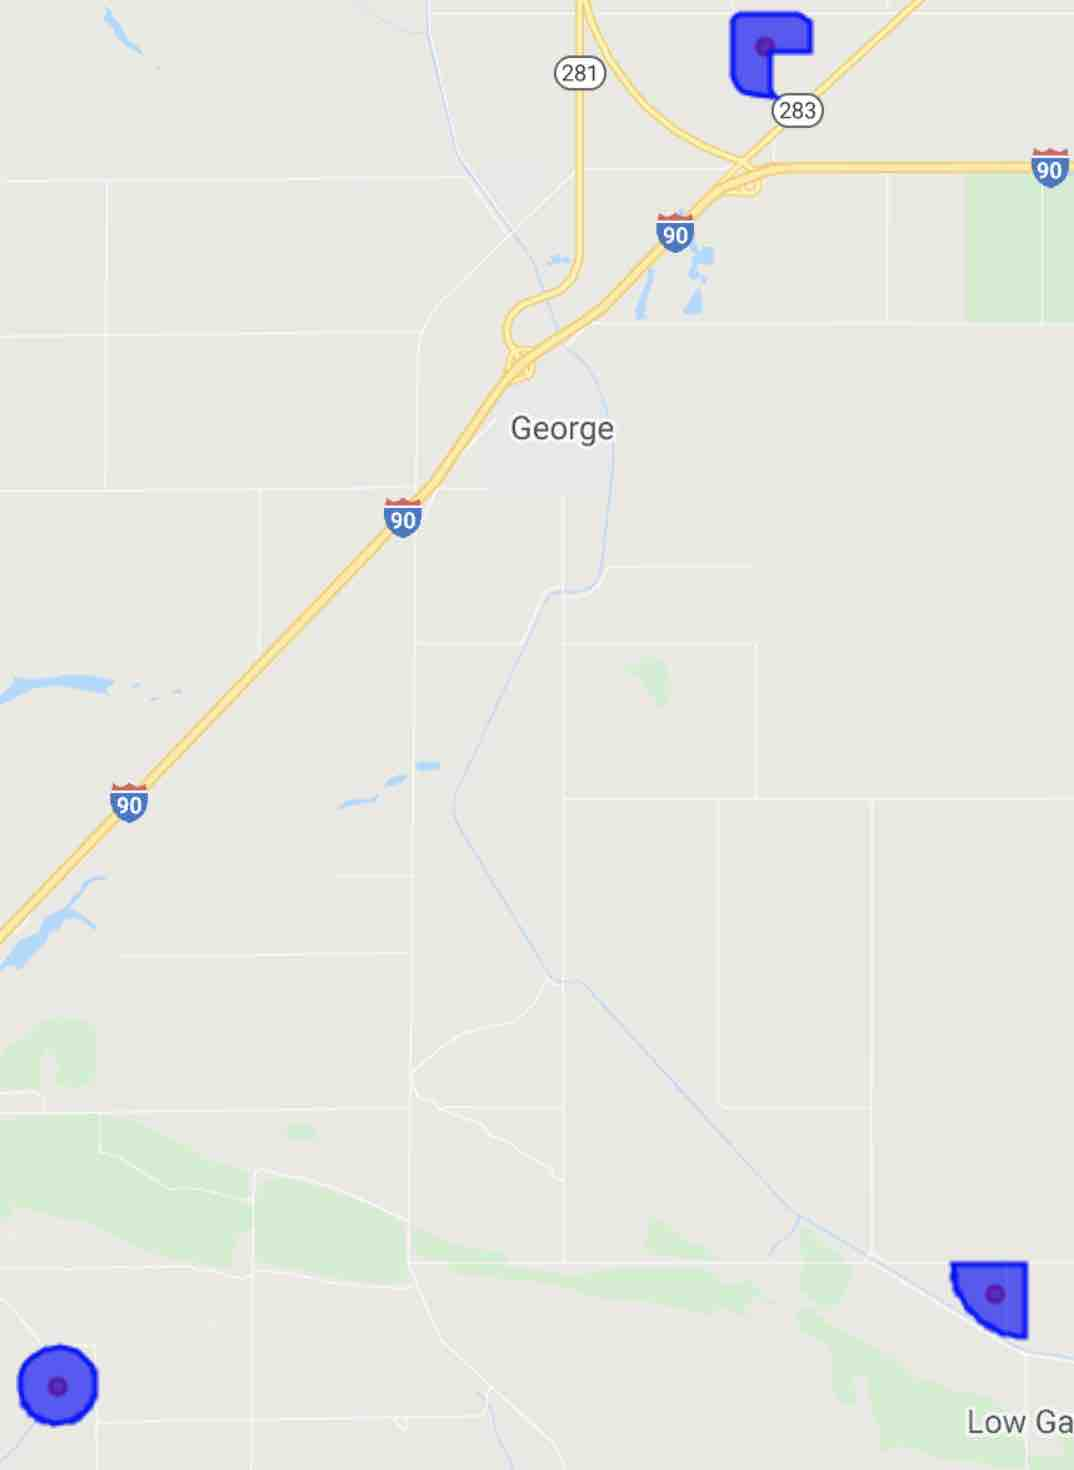
\includegraphics[width=1.1\textwidth]{figures/badCentroid}
    \caption{Bad Centroid}
    \label{fig:badCentroid}
  \end{subfigure}
  \qquad 
  \begin{subfigure}[b]{.4\textwidth}
    % \centering
    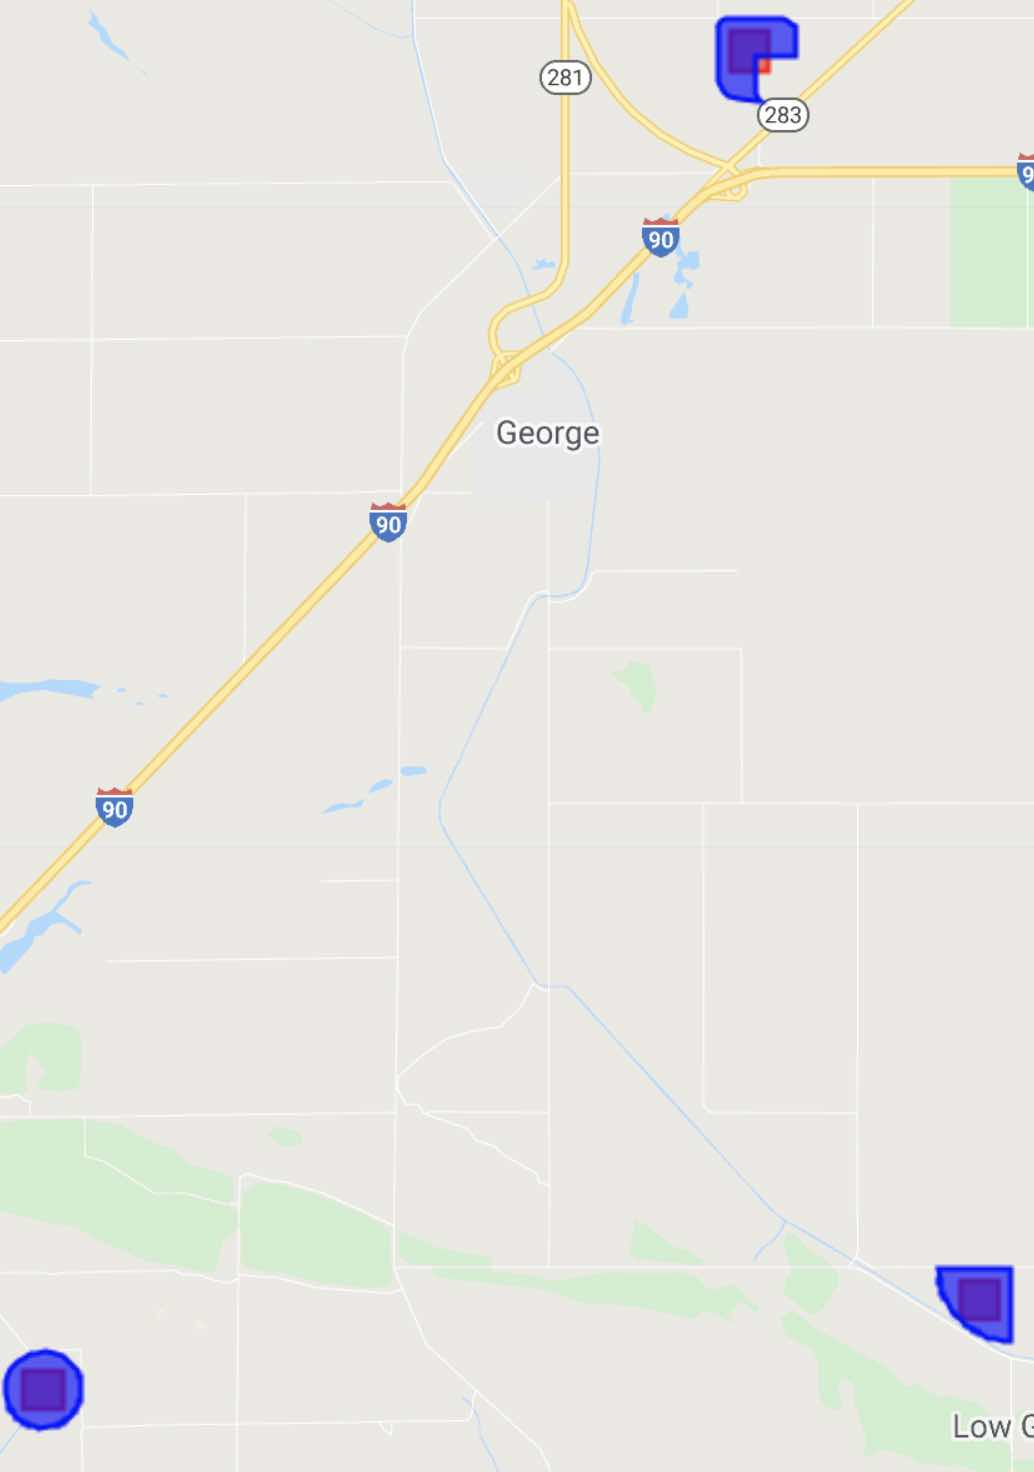
\includegraphics[width=1.06\textwidth]{figures/badBuffer}
    \caption{Bad Buffer}
    \label{fig:badBuffer}
  \end{subfigure}
\caption{Centroids and buffers around the centroids of 
         polygons in a shapefile.}
\label{fig:badPolygon}
\end{figure}
By adding one line (line 5.5 in Alg.~\ref{alg:FindCentroidsBuffers}) 
to the function \func{getCentroid(.)}
we can get a buffer (a rectangular or a circle area) around
the centroids.
\begin{tcolorbox}
  \begin{algorithm}[H]
  \label{alg:FindCentroidsBuffers}
   \caption{Make a Buffer Around Centroids of Polygons.}
\SetAlgoLined
% \KwResult{Faster convergence}
1. \textbf{function} 
\code{get\_rectangle\_arround\_centroid(feature)}\{ \\
  \vspace{.1in}
\hspace{.2in} 2.  {\color{ForestGreen}{// Keep this list of properties.}}\;
\hspace{.2in} 3. \textbf{var} \code{keepProperties} = [\codeRed{`ID'}, \codeRed{`county'}] \;
  \vspace{.2in}
\hspace{.2in} 4. {\color{ForestGreen}{// Get the centroid of the feature's geometry.}}\;
\hspace{.2in} 5. \textbf{var} 
\code{centroid} = 
\code{feature}.\func{geometry}().\func{centroid}(); \;
\vspace{.1in}
  
\hspace{.2in} 5.5 
\small{\code{centroid} =
\func{ee.Feature}(\code{centroid}.\func{buffer}(\codeCyan{200}).\func{bounds}())}\;

\vspace{.1in}
\hspace{.2in} 6. {\color{ForestGreen}{// Return a new Feature, copying properties from the
  
\hspace{.2in} old Feature.}}\;
\hspace{.2in} 7. \textbf{return} \func{ee.Feature}(\code{centroid}).\func{copyProperties}(\code{feature},
  
  \hspace{2.8in} 
  \code{keepProperties})\;
8. \}

  \vspace{.1in}
9. \textbf{var} \code{SF} =
\func{ee.FeatureCollection}(\code{Our\_ShapeFile})\;
10. \textbf{var}
\code{centroids\_from\_GEE} =  

\hspace{1.4in}
\code{SF}.\func{map}
(\code{get\_rectangle\_arround\_centroid});
\end{algorithm}
\end{tcolorbox}

%%%%%%%----------------------------------------
%%%%%%%
%%%%%%%       Cloud Filtering
%%%%%%%
\section{Cloud Filtering}
Handling clouds for Sentinel and Landsat are different. 
Let us start by \textbf{Sentinel}.\\

\noindent First, the followings are equivalent:

\begin{itemize}[leftmargin=0.5cm]
 \item  \textbf{var} \code{filtered = my\_IC}.\func{filterMetadata}(
    \codeRed{`CLOUDY\_PIXEL\_PERCENTAGE'},

    \hspace{2.5in} \codeRed{`less\_than'}, \codeRed{70});
    
    \item \textbf{var} \code{filtered = my\_IC}.\func{filter}(\codeRed{`CLOUDY\_PIXEL\_PERCENTAGE < 70'})
    
    \item \textbf{var} \code{filtered = my\_IC}.\func{filter}(\func{ee.Filter.lte}(\codeRed{`CLOUDY\_PIXEL\_PERCENTAGE'}, 
    
    \hspace{2.9in} \codeRed{70}))
\end{itemize}
\noindent They all filter out \emph{images} 
with cloud cover less than or equal to 70\%.
Those images will NOT be in our 
\code{filtered} collection.
Said differently, 
our \code{filtered} 
collection may include images that 
are covered by cloud up t0 70\%.

This is a pre-filtering step. Later, 
we can toss out the cloudy 
\emph{pixels} from every single image.

\begin{tcolorbox}
  \begin{algorithm}[H]
  \label{alg:FilterCloudyPixelsSentinel}
   \caption{Filter Cloudy Pixels for Sentinel.}
\SetAlgoLined
% \KwResult{Faster convergence}
1. \textbf{function} \code{maskS2clouds(image)} \{ \\
  \vspace{.2in}
\hspace{.2in} 2. {\color{ForestGreen}{// Each Sentinel-2 
                 image has a bitmask band with cloud 

\hspace{.55in} mask information QA60.}}\;
\hspace{.2in} 
3. \textbf{var} \code{qa = image}.\func{select}(\codeRed{`QA60'}); 

\vspace{.2in}
\hspace{.2in} 
4. {\color{ForestGreen}{// Bits 10 and 11 
                are clouds and cirrus, respectively.}}\;

\hspace{.2in} 5. \textbf{var} \code{cloudBitMask =} \codeCyan{1} $\code{<<}$ \codeCyan{10}  \;

\hspace{.2in} 6. \textbf{var} \code{cirrusBitMask =} \codeCyan{1} $\code{<<}$ \codeCyan{11} \;

\vspace{.2in}
\hspace{.2in} 7. 
{\color{ForestGreen}{// Both flags 
should be set to zero, 
indicating clear 

\hspace{.6in} conditions.}}\;

\hspace{.2in} 8. 
\textbf{var} \code{mask = qa}.\func{bitwiseAnd}(\code{cloudBitMask})
                  .\func{eq}(\codeCyan{0}).\func{and}(

\hspace{1.1in}     \code{qa}.\func{bitwiseAnd}(\code{cirrusBitMask})
                   .\func{eq}(\codeCyan{0}))\;

\vspace{.2in}
\hspace{.2in} 9. {\color{ForestGreen}{// Return the masked 
                 and scaled data, without 
        
                  \hspace{.7in} the QA bands.}}

\hspace{.2in} 10. 
\textbf{return}
\code{image}.\func{updateMask}(\code{mask})

\hspace{1.25in}
.\func{divide}(\codeCyan{10000})
                
\hspace{1.25in}
.\func{select}(\codeRed{``B.*''})
                
\hspace{.4in} .\func{copyProperties}(
                \code{image}, [\codeRed{``system:time\_start''}]);
                
\hspace{.01in} 11. \}
\end{algorithm}
\end{tcolorbox}

\noindent \textbf{{\color{red}{Note 1:}}} Please note
the last line in Alg.~\ref{alg:FilterCloudyPixelsSentinel}
is copying the system start time into the image which
has nothing to do with clouds. It may be handy later.\\


\noindent \textbf{{\color{red}{Note 2:}}} Please note
the three (equivalent) pre-filtering of images mentioned 
above do not exist for Landsat!\\

Landsat(s) is a different satellite, and 
therefore, the cloud filtering must 
be handled
differently; the band names that includes 
cloud information are different 
between Sentinel and
Landsat or even among different Landsats.\\

Landsat-8 \emph{Surface Reflectance} cloud mask~\cite{Landsat8CloudMask}:
\begin{tcolorbox}
  \begin{algorithm}[H]
  \label{alg:FilterCloudyPixelsLandsat8}
   \caption{Filter Cloudy Pixels for Landsat-8 \textbf{Tier 1 and 2} \emph{Surface Reflectance}.}
\SetAlgoLined
% \KwResult{Faster convergence}
1. \textbf{function} 
\code{maskL8sr(image)} \{\\

\vspace{.1in}

\hspace{.2in} 2. 
{\color{ForestGreen}{// Bits 3 and 5 are cloud 
shadow and cloud, 

\hspace{.55in} respectively.}}\;

\hspace{.2in} 3. \textbf{var}
\code{cloudShadowBitMask} =
(\codeCyan{1} $\code{<<}$ \codeCyan{3})\;
\hspace{.2in} 4. \textbf{var} \code{cloudsBitMask} = (\codeCyan{1} $\code{<<}$ \codeCyan{5})\;

\vspace{.2in}  
\hspace{.2in} 5. {\color{ForestGreen}{// Get the pixel QA band.}}\;

\hspace{.2in} 6.  
\textbf{var} \code{qa =} \code{image}.\func{select}(\codeRed{`pixel\_qa'})\;

\vspace{.2in}
\hspace{.2in} 7. {\color{ForestGreen}{// Both flags should be set to zero, indicating clear 

\hspace{.5in}  conditions.}}\;

\hspace{0.2in} 8. {\small{
\textbf{var} \code{mask = }
          \code{qa}.\func{bitwiseAnd}(\code{cloudShadowBitMask})
          .\func{eq}(\codeCyan{0})
          
\hspace{1.25in} .\func{and}(\code{qa}.\func{bitwiseAnd}(\code{cloudsBitMask}).\func{eq}(\codeCyan{0}))}}\;

\vspace{.2in}
\hspace{.2in} 9. \textbf{return}
\code{image}.\func{updateMask}(\code{mask})\;
  
\hspace{.01in} 10. \}
\end{algorithm}
\end{tcolorbox}

\noindent \textbf{{\color{red}{Note:}}} This is
written for Landsat-8 (Surface Reflectance Tier 1 and 2).\\


The code for masking the cloudy pixels in Landsat-4, 5, and 7 
\emph{Surface Reflectance} is given by~\cite{Landsat457CloudMask}
that is given below by Alg.~\ref{alg:FilterCloudyPixelsLandsat457}:
\begin{tcolorbox}
  \begin{algorithm}[H]
  \label{alg:FilterCloudyPixelsLandsat457}
   \caption{Filter Cloudy Pixels for Landsat-4, 5, and 7 \textbf{Tier 1 and 2} \emph{Surface Reflectance}.}
\SetAlgoLined
% \KwResult{Faster convergence}

1. \textbf{function} 
\code{cloudMaskL457(image)} \{

\vspace{.1in}
\hspace{.2in} 2. 
\textbf{var} \code{qa = image}.\func{select}(\codeRed{`pixel\_qa'})\;

\vspace{.1in}
\hspace{.2in} 3. {\color{ForestGreen}{// If the cloud bit (5) is set and
                      the cloud confidence (7) 
                      
\hspace{0.6in}   is high or the cloud shadow bit is set (3), 


\hspace{0.6in}        then it's a bad pixel.}}\\

\hspace{.2in} 4. 
\textbf{var} 
\code{cloud = qa}.\func{bitwiseAnd}(\codeCyan{1} $\code{<<}$ \codeCyan{5})\\
\hspace{1.35in}   .\func{and}(\code{qa}.\func{bitwiseAnd}(\codeCyan{1} $\code{<<}$ \codeCyan{7}))\\
\hspace{1.35in}   .\func{or}(\code{qa}.\func{bitwiseAnd}(\codeCyan{1} $\code{<<}$ \codeCyan{3}))\;

\vspace{.1in} 

\hspace{.2in} 5.
{\color{ForestGreen}{// Remove edge pixels that don't occur in all bands}}\\

\hspace{.2in} 6.
\textbf{var} 
\code{mask2 = image}.\func{mask}().\func{reduce}(\func{ee.Reducer.min}())\;

\hspace{.2in} 7.
\small{\textbf{return} \code{image}.\func{updateMask}(\code{cloud}.\func{not}()).\func{updateMask}(\code{mask2});}
  
\hspace{.01in} 10. \}
\end{algorithm}
\end{tcolorbox}

I have copied the cloud masking functions
from GEE development/data-product pages into a script that can be found 
\href{https://code.earthengine.google.com/?scriptPath=users\%2Fhnoorazar\%2FGEE_Mini_Tutorial\%3ACloudMaskings}{here}~\cite{CloudandMaskingFunctionsonMyGEE}.
More on masking clouds of Sentinel-2 and shadows
are provided \href{https://developers.google.com/earth-engine/tutorials/community/sentinel-2-s2cloudless}{here} by GEE developers~\cite{CloudandShadowSentinel}.


%%%%%%%----------------------------------------
%%%%%%%
%%%%%%%     Timelines
%%%%%%%
\section{Timelines}
\label{sec:Timelines}
Figure~\ref{fig:landsatTimeline}
shows the timeline of Landsat
satellites~\cite{LandsatTimelinesWiki}
and~\cref{tab:ElevationTable} shows the
exact dates.
\begin{figure}[H]
  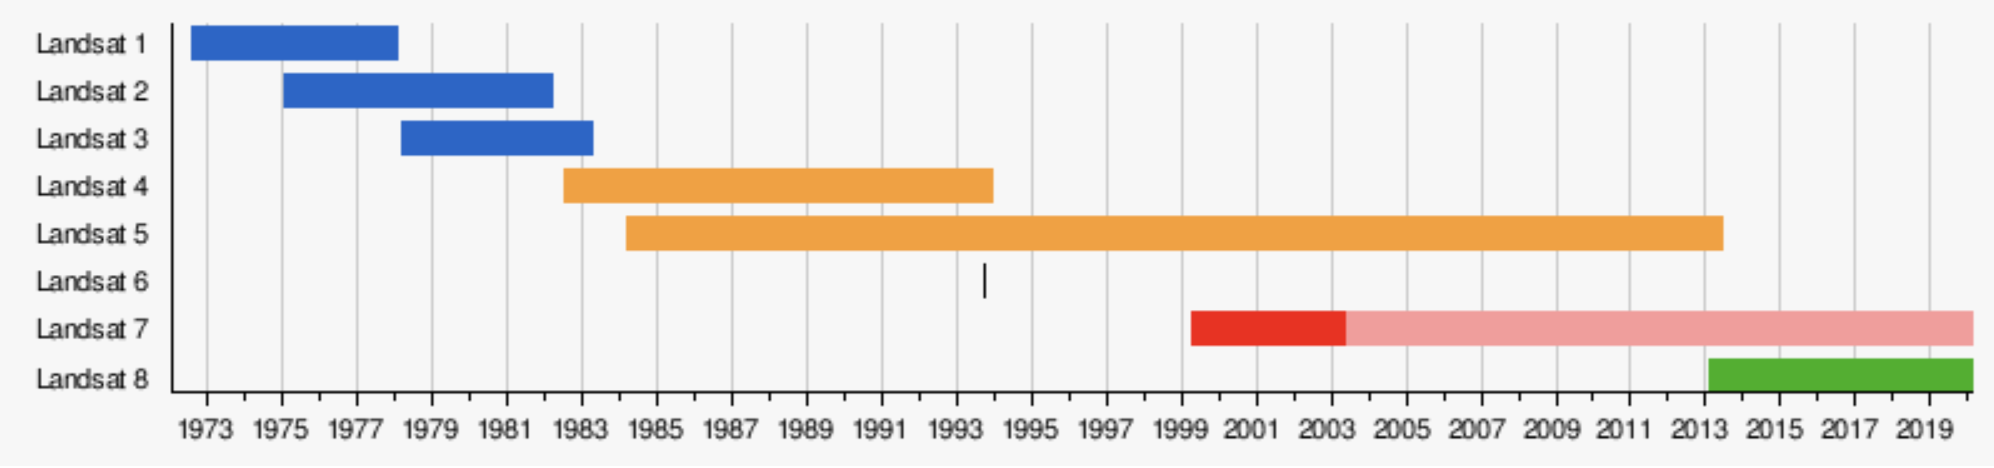
\includegraphics[width=1\textwidth]{figures/landsatTimeline1}
\caption{Landsat Timeline.}
\label{fig:landsatTimeline}
\end{figure}

\begin{table}[]
\centering
\caption{Landsat timeline table.} 
\label{tab:ElevationTable}
\begin{tabular}{|l|l|l|}
\hline
\rowcolor{shadecolor} 
\small{Satellite} & 
\small{Launched} & 
\small{Terminated} \\
\hline
Landsat 5 & 1 March 1984 & 5 June 2013 \\ 
\hline
\rowcolor{aliceblue} 
Landsat 6 & 5 October 1993  & 5 October 1993 \\ \hline
Landsat 7 & 15 April 1999 & Still active \\ \hline
\rowcolor{aliceblue} 
Landsat 8 & 11 February 2013 & Still active \\ \hline
Landsat 9 & 16 September 2021 (planned) & - \\ \hline
\end{tabular}
\end{table}

%%%%%%%----------------------------------------
%%%%%%%
%%%%%%%     Band Names and Indices
%%%%%%%
\section{Band Names and Indices}
\label{sec:Band_Names_and_Indices}

Band names are different in each instrument
(see~\cref{tab:BandNameTable}).
Hence the indices must be defined differently
using proper band names.
Below we see some of indices.
\cref{tab:SomeBandWavelengths} also provides
more insight about the bandwidths of the satellites.
The bandwidths are very similar. If their
minimal differences makes any difference I am not aware of it and do not care. 
Go nuts if you wish; figure out why, what, how.
Bandwidths of Sentinel-2 is found on Wikipedia~\cite{SentinelBandwidths}
and Bandwidths of Landsats can be found on GEE pages (e.g.~\cite{Landsat7T1SRBandWidths}).

\begin{table}[]
\centering
\caption{Some Band Names in Satellites.} 
\label{tab:BandNameTable}
\begin{tabular}{|l|l|l|l|}
\hline
\rowcolor{shadecolor} 
\small{Satellite} & 
\small{NIR} & 
\small{Red}  &
\small{Blue} \\
\hline
Sentinel & B8 & B4 & B2\\ 
\hline
\rowcolor{aliceblue} 
Landsat-8 & B5 & B4 & B2\\ 
\hline
Landsat-7 & B4 & B3 & B1\\ 
\hline
\rowcolor{aliceblue} 
Landsat-5 & B4 & B3 & B1\\ 
\hline
\end{tabular}
\end{table}


\begin{table}[]
\centering
\caption{Some Band Wavelengths. The bandwidths are very similar. If their
minimal differences makes any difference I am not aware of it and do not care. 
Go nuts if you wish; figure out why, what, how.} 
\label{tab:SomeBandWavelengths}
\begin{tabular}{|l|l|l|l|}
\hline
\rowcolor{shadecolor} 
\small{Satellite} & 
\small{NIR} & 
\small{Red}  &
\small{Blue} \\
\hline
Sentinel-2A & B8:~~~~~~0.77 -- 0.88 $\mu m$ & B4:~~~~~~0.65 -- 0.68 $\mu m$ & B2:~~~~~~0.46 -- 0.52 $\mu m$\\ 
\hline
\rowcolor{aliceblue} 
Sentinel-2B & B8:~~~~~~0.78 -- 0.88 $\mu m$ & B4:~~~~~~0.65 -- 0.68 $\mu m$ & B2:~~~~~~0.46 -- 0.52 $\mu m$ \\ 
\hline
Landsat-8 & B5:~~~~~~0.85 -- 0.88 $\mu m$ & B4:~~~~~~0.64 -- 0.67 $\mu m$ & B2:~~~~~~0.45 -- 0.51 $\mu m$\\ 
\hline
\rowcolor{aliceblue} 
Landsat-7 & B4:~~~~~~0.77 -- 0.90 $\mu m$ & B3:~~~~~~0.63 -- 0.69 $\mu m$ & B1:~~~~~~0.45 -- 0.52 $\mu m$\\ 
\hline
Landsat-5 & B4:~~~~~~0.77 -- 0.90 $\mu m$  & B3:~~~~~~0.63 -- 0.69 $\mu m$ & B1:~~~~~~0.45 -- 0.52 $\mu m$\\ 
\hline
\rowcolor{aliceblue} 
Landsat-7 C2 L2 & SR\_B4: 0.77 -- 0.90 $\mu m$ & SR\_B3: 0.63 -- 0.69 $\mu m$ & SR\_B1: 0.45 -- 0.52 $\mu m$\\ 
\hline
Landsat-5 C2 L2 & SR\_B4: 0.77 -- 0.90 $\mu m$ & SR\_B3: 0.63 -- 0.69 $\mu m$ & SR\_B1: 0.45 -- 0.52 $\mu m$\\ 
\hline
\end{tabular}
\end{table}





\begin{gather}
\label{eq:EVILandsat8}
\begin{aligned}
\EVI &= G \times \frac{\NIR - R}{\NIR + C1 \times R - C2 \times B + L} \\
\EVI_S &= 2.5 \times \frac{B8 - B4}{B8 + 6 \times B4 - 7.5 \times B2 + 1}\\
\EVI_8 &= 2.5 \times \frac{B5 - B4}{B5 + 6 \times B4 - 7.5 \times B2 + 1} \\
\EVI_7 &= 2.5 \times \frac{B4 - B3}{B4 + 6 \times B3 - 7.5 \times B1 + 1}
\end{aligned}
\end{gather} 

\noindent where $NIR$ is near infrared, $R$ is Red,
$B$ is blue, 
$\text{EVI}_8$ is the Enhanced Vegetation Index (EVI) 
in Landsat-8~\cite{Landsat8EVI}, 
and $\text{EVI}_S$
is the EVI in Sentinel; The NIR band in
Landsat-8 is $B5$~\cite{L8BandNames}
and for Sentinel is $B8$.

``EVI is similar to Normalized Difference 
Vegetation Index (NDVI) and can be used 
to quantify vegetation greenness. However, 
EVI corrects for some atmospheric conditions 
and canopy background noise and is more 
sensitive in areas with dense vegetation. 
It incorporates an ``$L$'' value to adjust for 
canopy background, ``$C$'' values as coefficients 
for atmospheric resistance, and values from 
the blue band ($B$).  These enhancements allow 
for index calculation as a ratio between 
the $R$ and $NIR$ values, while reducing the 
background noise, atmospheric noise, and 
saturation in most cases''~\cite{Landsat8EVI}.

Below are the NDVIs for 
Landsat-4 to Landsat-7~\cite{Landsat4NDVI},
Landsat-8~\cite{Landsat4NDVI}, and Sentinel:
\begin{gather}
\label{eq:NDVILandsat8}
\begin{aligned}
\text{NDVI} &= \frac{NIR - R}{NIR + R}\\
\text{NDVI}_S &= \frac{B5 - B4}{B5 + B4}\\
\text{NDVI}_8 &= \frac{B8 - B4}{B8 + B4} \\
\text{NDVI}_{4-7} &= \frac{B4 - B3}{B4 + B3} \\
\end{aligned}
\end{gather}

Landsat-7 has 8-day NDVI composite already provided 
by GEE~\cite{Landsat7NDVIComposite}. This product
is based on TOA data which is not perfect! However,
it seems running some smoothing methods on it can
make it useful.


\section{Tiny Tips, Big Problems}
\label{sec:Tiny-Tips-Big-Problems}

Some times you may find yourself in a situation
for which you are using the biggest sledgehammer to deal
with the tiniest nail. In these scenarios the empire of Google
does not have a function (for good reasons most likely) to do the job. 
If brute force is the chosen approach these tips may help.

\begin{description}
\item [Object Types] There are two types of objects or functions.
Some are called server-side. Some are called client-side.
Here is an \href{https://code.earthengine.google.com/?scriptPath=users\%2Fhnoorazar\%2FGEE_Mini_Tutorial\%3AobjectTypeForLoop}{example}  
that shows a client-side object does not work with server-side object.

It is strongly advised to avoid using/writing client-side
objects/functions. The client-side objects also make the
server/code/interface be very slow, freeze at times.

\item [Batch Export] This is an example that Google does not think
is useful. But if you need to export a collection of images you can do it
either using a for-loop for which you may need to look at the previous example.
Or, you can use \func{batch.Download.ImageCollection.toDrive(.)}. 
Both of these approaches are demonstrated \href{https://code.earthengine.google.com/cda913b68aecf6e49b3d09961c1cd458}{here}.

Two remarks in this regard. First, the function for downloading the image 
collection as a batch\footnote{\func{batch.Download.ImageCollection.toDrive(.)}} did not work for me,
but the for-loop did\footnote{I was visualizing the images as RGB images and exporting them; \textbf{var} \code{imageRGB =} \codeCyan{an\_image}.\func{visualize}(vizParams). 
I am not too sure if the batch download's problem is specific to RGB images.}.
The images I exported turned out to be black and white.
Secondly, any time a data is exported on GEE interface, you need
to click on the \textbf{Run} button on \textbf{Task} tab. Perhaps Python
can be used to avoid this problem, as well as server-side/client-side
problem altogether.


\end{description}



%%%%%%%----------------------------------------
%%%%%%%
%%%%%%% references
%%%%%%%

\bibliographystyle{unsrt}
\bibliography{GEE_References.bib}

%%%%%%%----------------------------------------
%%%%%%%
%%%%%%%       The End
%%%%%%%
\end{document}
